This section details the experimental methodology, including the dataset employed, the procedures for data pre-processing and synthetic fault injection, and the architecture of our proposed Hierarchical Fault Identification Network (HiFiNet) for fault classification in WSNs.

\subsection{Fault Injection}
To evaluate the performance of HiFiNet in classifying various fault types, synthetic faults were injected into the pre-processed normal temperature data.

For each experimental dataset used, faults were injected such that within the selected subset of six nodes, five nodes were each assigned a distinct fault type, and one node remained normal. This setup allows for the analysis of one specific fault type per sensor in the context of other faulty and normal sensors.

Multiple datasets were generated with varying overall percentages of faulty instances, specifically 5\%, 10\%, 15\%, and 20\% of the total data points being faulty. Within each dataset, the total fault rate was divided equally among the five predefined fault types. Faults were injected based on their mathematical models Equation \ref{eq:hardover}, \ref{eq:drift}, \ref{eq:spike}, \ref{eq:erratic}, and \ref{eq:stuck}. In total, 4 datasets are created from each original dataset corresponding to each fault rate.

The time series sequences were labeled with a specific fault type if any sample within that sequence contained the corresponding injected fault. This creates a labeled dataset suitable for supervised learning.

\subsection{Hierarchical Fault Identification Network (HiFiNet)}
\begin{figure}
  \centering
  \includegraphics[width=0.8\linewidth]{images/HiFiNet.png}
  \caption{Proposed HiFiNet model, illustrating the Edge Classifier processing a target node's temperature sequence and the Network Classifier integrating edge outputs with contextual network data.}
  \label{fig:hifinet}
\end{figure}
We propose HiFiNet, a Hierarchical Fault Identification Network, for the classification of sensor faults in WSNs. The architecture, depicted in Figure~\ref{fig:hifinet}, employs a two-stage hierarchical approach to classify faults, leveraging both individual sensor data and contextual information from the network.

\subsubsection{Edge Classifier}
The first stage of HiFiNet is the Edge Classifier, which focuses on analyzing the time series data from an individual target sensor node to extract discriminative features and perform an initial fault classification. The design of the Edge Classifier involves a two-phase training process: unsupervised pre-training of a feature extractor using a LSTM-SAE architecture, followed by supervised fine-tuning for the fault classification task.

The feature-extraction component is built from an LSTM-SAE with encoder layers. In the first phase, this autoencoder is trained in an unsupervised, layer-wise fashion to learn compressed representations of \(X_w\). Define \(E_l(\cdot; \theta_{E_l})\) as the \(l\)-th LSTM encoder layer with parameters \(\theta_{E_l}\), \(D_l(\cdot; \theta_{D_l})\) as the corresponding decoder layer with parameters \(\theta_{D_l}\), and \(H_l\) as the hidden representation output by \(E_l\). We have:
\begin{itemize}
  \item \emph{Layer \(l=1\):}
    \begin{equation}
      \begin{aligned}
        H_1 &= E_1(X_w; \theta_{E_1}), \\
        \hat X_w &= D_1(H_1; \theta_{D_1}), \\
      \end{aligned}
    \end{equation}
    with \(\hat X_w\) being the reconstructed input. Then the objective is to optimize the reconstruction loss with respective to the network parameters:
    \begin{equation}
      (\hat \theta_{E_1},\,\hat \theta_{D_1}) = \underset{\theta_{E_1}, \theta_{D_1}} {\arg\min} \mathcal L_{\text{recon}}(X_w; \hat X_w)
    \end{equation}
  \item \emph{Layer \(l = 2, \ldots, L\)}

    Define \(H^*_{l-1}\) as the output of the \((l-1)\)-th trained encoder layer. We have:
    \begin{equation}
      \begin{aligned}
        H_l &= E_l(H^*_{L-1}; \theta_{E_l}), \\
        \hat H^*_{l-1} &= D_l(H_l; \theta_{D_l}), \\
      \end{aligned}
    \end{equation}
    with \(\hat H^*_{l-1}\) being the reconstructed input. Again the objective is to optimize the reconstruction loss with to the network parameters:
    \begin{equation}
      (\hat \theta_{E_l},\,\hat \theta_{D_l}) = \underset{\theta_{E_l}, \theta_{D_l}} {\arg\min} \mathcal L_{\text{recon}}(H^*_{l-1}; \hat H^*_{l-1})
    \end{equation}
\end{itemize}
After all \(L\) layers are pre-trained, the full stacked LSTM encoder is formed by concatenating these trained layers: \(E_\text{stacked}(\cdot; \Theta^*_{E}) = E_L(\ldots E_1(\cdot; \theta^*_{E_L}) \ldots;\theta^*_{E_L})\)

The pre-trained stacked LSTM encoder, \(E_\text{stacked}\), now served as the feature extractor for the Edge Classifier. In the second phase, classification head is attached to this encoder to create the Edge Classifier. The complete network is then trained using the labeled dataset.

\subsubsection{Iterative Graph Network}
The second stage of HiFiNet is the Network Classifier, which refines the initial fault assessments or embeddings from the Edge Classifier by incorporating network-wide spatial context and inter-node dependencies. The core of the Network Classifier is an IGN. Figure~\ref{fig:ign} depicts the information flow in an IGN.

\begin{figure}
  \centering
  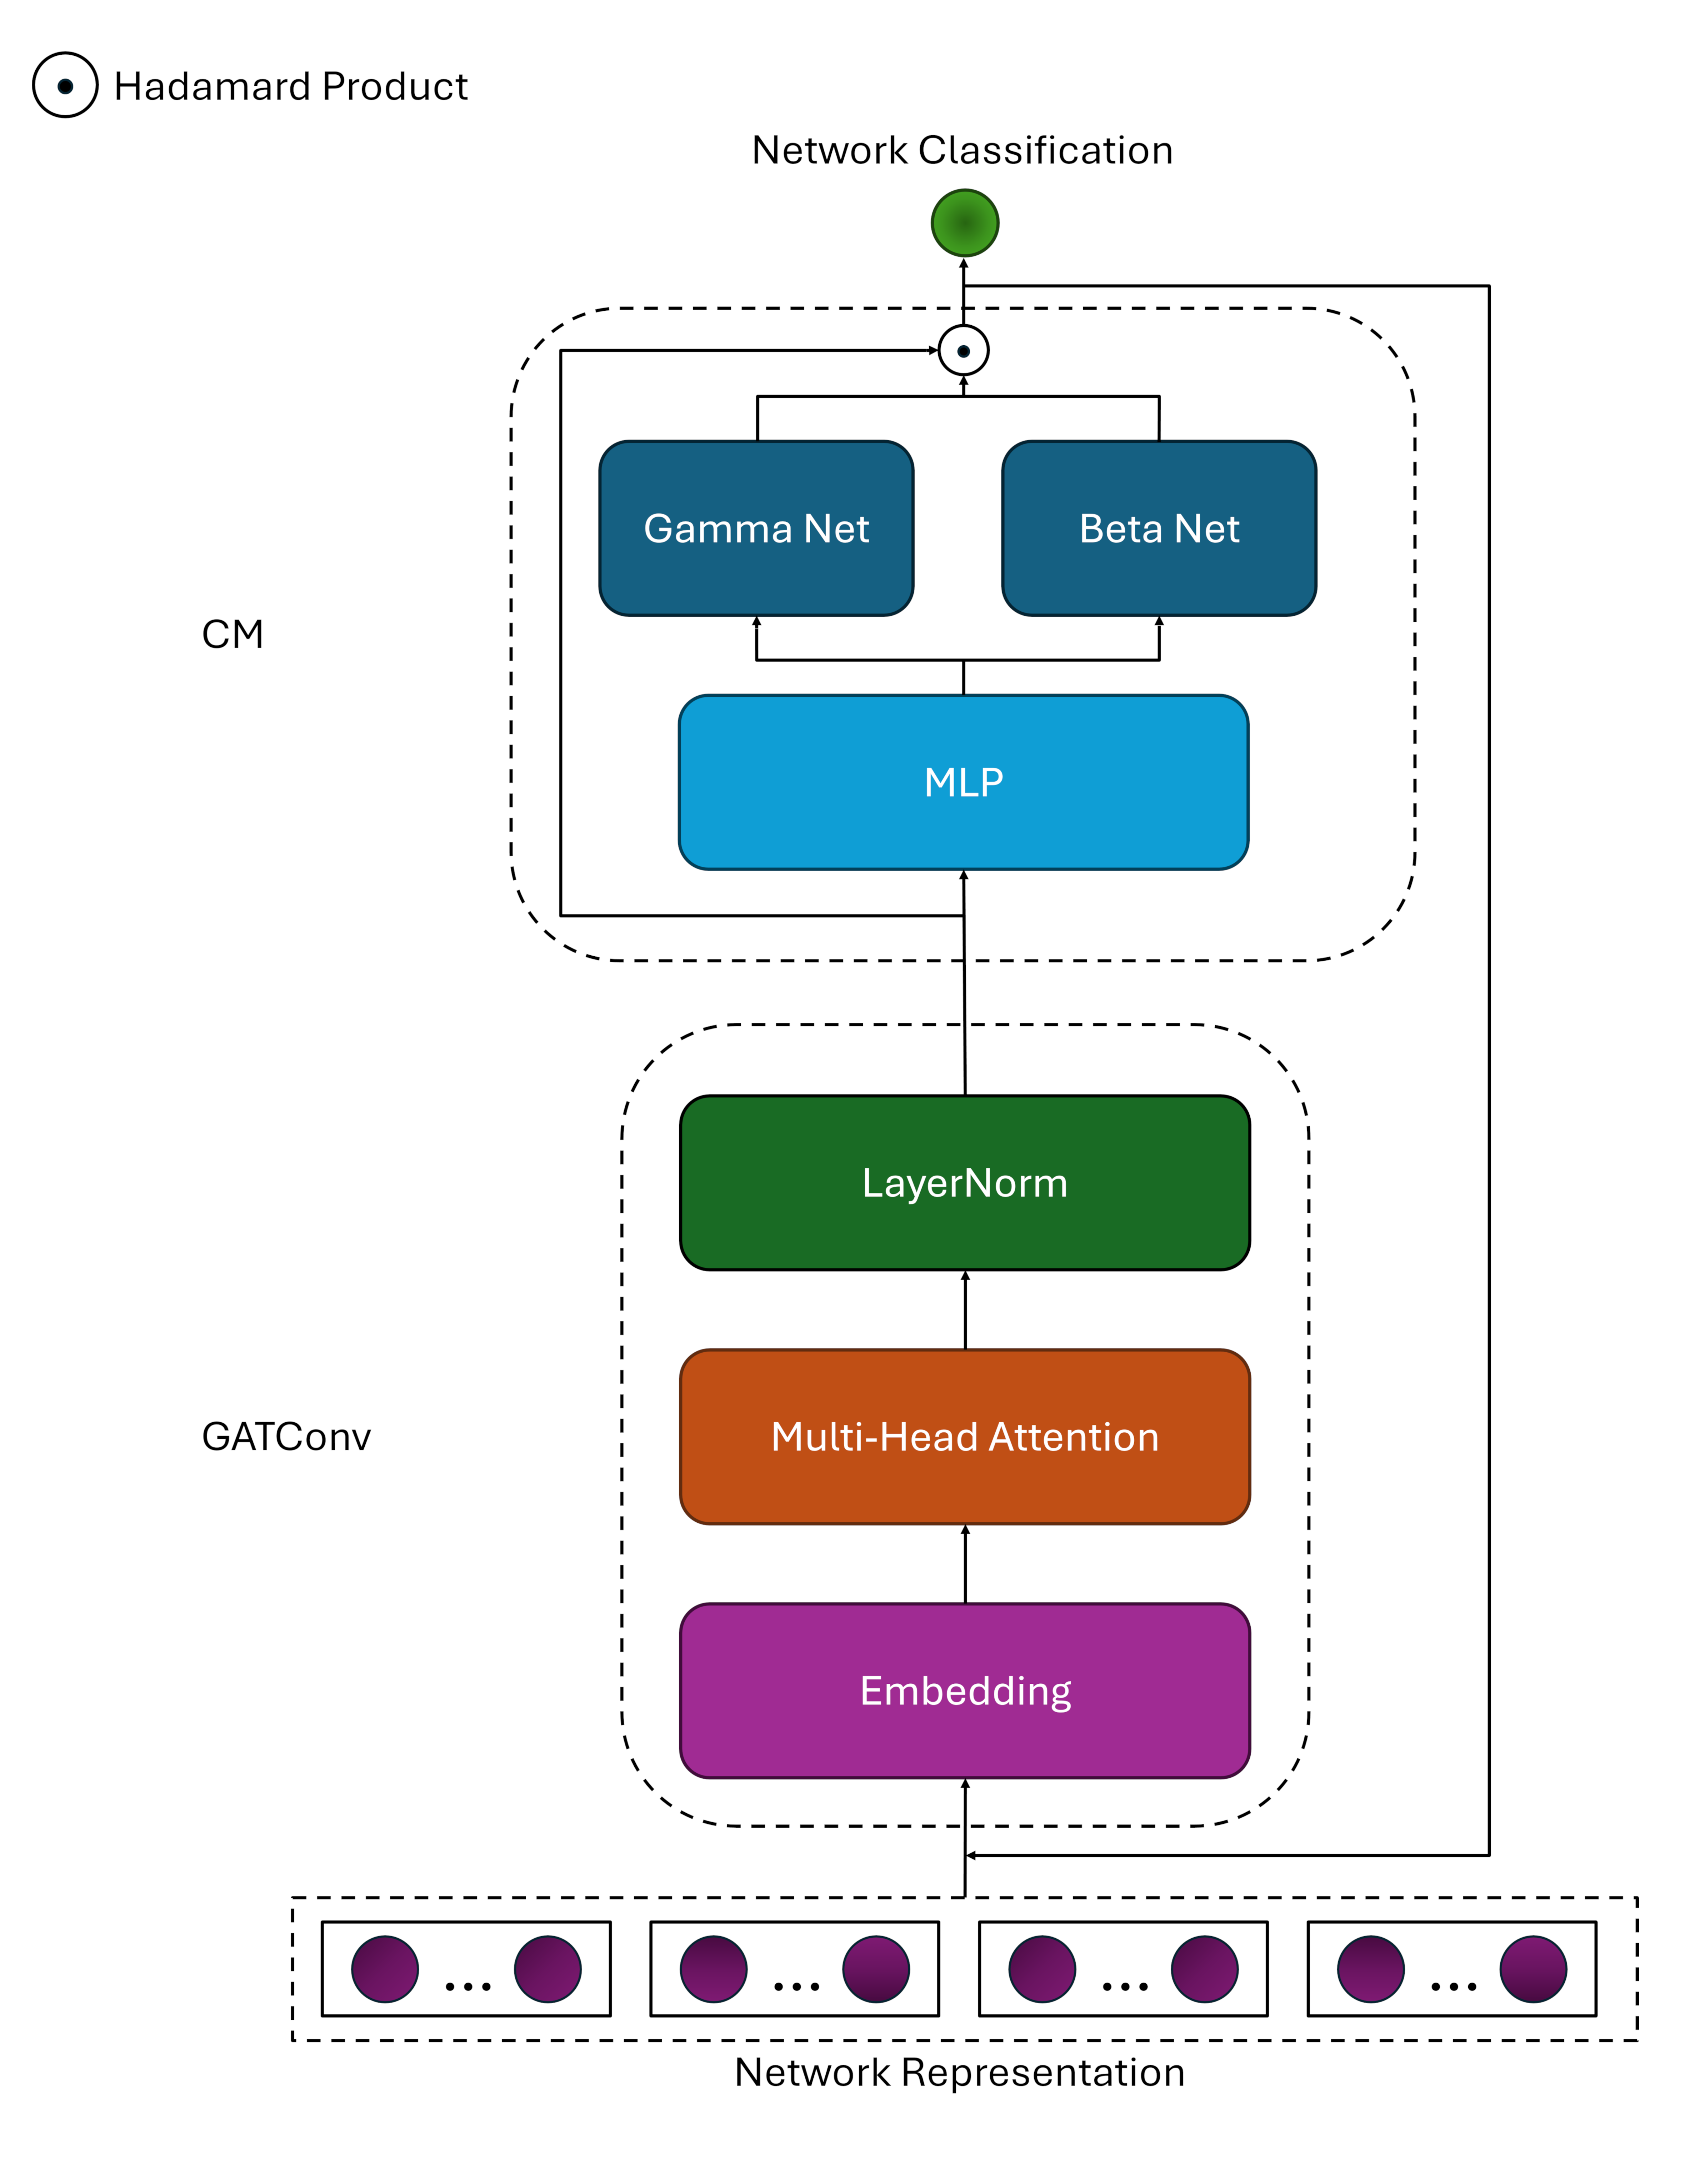
\includegraphics[width=0.8\linewidth]{images/IGN.png}
  \caption{Illustration of the Iterative Graph Network architecture, showing the iterative process of feature modulation, graph attention convolution, and confidence update.}
  \label{fig:ign}
\end{figure}

The IGN is designed to dynamically refine node representations by iteratively propagating and aggregating information across the graph, modulated by an evolving confidence measure. Let \(\mathcal{H}^{(0)} \in \mathbb{R}^{N \times d_0}\) be the vector representation of a node with \(N\) is the number of nodes and \(d_0\) is the dimension of the edge output. The IGN performs \(K\) iterations.

In each iteration \(k = 0, \dots, K\):
\begin{itemize}
  \item Feature Modulation (for \(k > 0\)):
    The initial node embeddings $\mathbf{H}^{(0)}$ are modulated based on a confidence score vector \(\mathbb{c}^{(k-1)} \in \mathbb{R}^{N \times 1}\), derived from the \((k-1)\)-th iteration's GAT output. A Confidence Modulator function, $\mathcal{M}_{\text{c}}$, is employed using Feature-wise Linear Modulation (FiLM):
    \begin{equation}
      \mathcal{H}'^{(k)} = \mathcal{M}_{\text{c}}(\mathcal{H}^{(0)}, \mathbb{c}^{(k-1)}) = g_{\gamma}(c^{(k-1)}) \odot \mathcal{H}^{(0)} + g_{\beta}(c^{(k-1)})
    \end{equation}
    where \(g_{\gamma}(\cdot)\) and \(g_{\beta}(\cdot)\) are learnable functions that generate scaling and shifting parameters from the confidence scores, and \(\odot\) denotes element-wise multiplication. For the first iteration \(k=0\), no modulation is applied, so \(\mathcal{H}'^{(0)} = \mathcal{H}^{(0)}\). The Confidence Modulator allows the network to adaptively emphasize or de-emphasize features based on the current confidence in their classification.

  \item Graph Attention Convolution (GAT) Block:
    The modulated features \(\mathbb{H}'^{(k)}\) are then processed by a GAT block, denoted as \(\mathcal{G}\). This block typically consists of one or more Graph Attention Convolution layers, which enable nodes to selectively attend to their neighbors' features when updating their own representations:
    \begin{equation}
      \mathcal{H}_{\text{G}}^{(k)} = \mathcal{G}(\mathcal{H}'^{(k)}, A)
    \end{equation}
    where \(A\) is the adjacency matrix representing the graph structure. Each GAT layer computes attention coefficients for neighboring nodes, aggregates their features weighted by these coefficients, and applies a linear transformation. Layer normalization and activation functions  are often applied between GAT layers. Dropout are also used for regularization. The output \(\mathcal{H}_{\text{G}}^{(k)} \in \mathbb{R}^{N \times d_{\text{G}}}\) contains node representations that have incorporated information from their local graph neighborhood.

  \item Temporary Classification and Confidence Update (if \(k < K-1)\):
    If it is not the final iteration, the output \(\mathcal{H}_{\text{G}}^{(k)}\) is passed through a temporary classifier, \(f_{\text{temp}}\), to obtain intermediate class logits \(z^{(k)}\) for each node:
    \begin{equation}
      z^{(k)} = f_{\text{temp}}(\mathcal{H}_{\text{G}}^{(k)})
    \end{equation}
    These logits are converted to probabilities $P^{(k)}$ using the softmax function:
    \begin{equation}
      P^{(k)} = \text{softmax}(\mathbf{z}^{(k)})
    \end{equation}
    The confidence score $c_i^{(k)}$ for each node $i$ is then derived from these probabilities, typically as the maximum probability value:
    \begin{equation}
      c_i^{(k)} = \max(P_i^{(k)})
    \end{equation}
    This results in a confidence vector $\mathbf{c}^{(k)}$, which is then used in the Feature Modulation step of the next iteration ($k+1$). This iterative process allows the model to progressively refine its understanding by focusing subsequent GAT operations based on the certainty of intermediate predictions.
\end{itemize}

After \(K\) iterations, the final GAT output $\mathcal{H}_{\text{G}}^{(K_{iter}-1)}$ represents the spatially-refined node embeddings. This and the original representation are then passed to a classification head to output the network classification.
